\documentclass{article}
\usepackage{caption}
\usepackage{cancel}
\usepackage[fontsize=16pt]{fontsize}
\usepackage{amsmath}
\usepackage{polynom}
\usepackage{longdivision}
\usepackage{tikz}
\usepackage[raggedrightboxes]{ragged2e}
\usepackage{tabularx}

\author{}
\date{}
\title{simple\\Division\\Course\\
\vspace{28pt}
\begin{center}
\includegraphics[width=4em]{ApS_logo.png}
\end{center}
\begin{normalsize}Tutoring Centre Ferndale\end{normalsize}}

\newcommand\mylongdiv[2]{%
$\strut#1$\kern.25em\smash{\raise.3ex\hbox{$\big)$}}$\mkern-8mu
        \overline{\quad\strut#2}$}

\setcounter{secnumdepth}{0}
\begin{document}
\maketitle

\section{Division}

Division means sharing equally.\\

\begin{enumerate}

\item What is division, in your own words?
\item Use division in a sentence.

\subsection{The Two Ways of Dividing}

\subsubsection*{Dividing into groups of equal size}

One way of dividing is when you have a number and you divide a larger number into as many pieces as you can of that size.

Say you were packing things into boxes and each box could hold 4 things. You would keep taking 4 things and packing them into boxes until you didn't have enough left for a full box. If you had 50 things you would have 12 full boxes with 2 things left over.\\

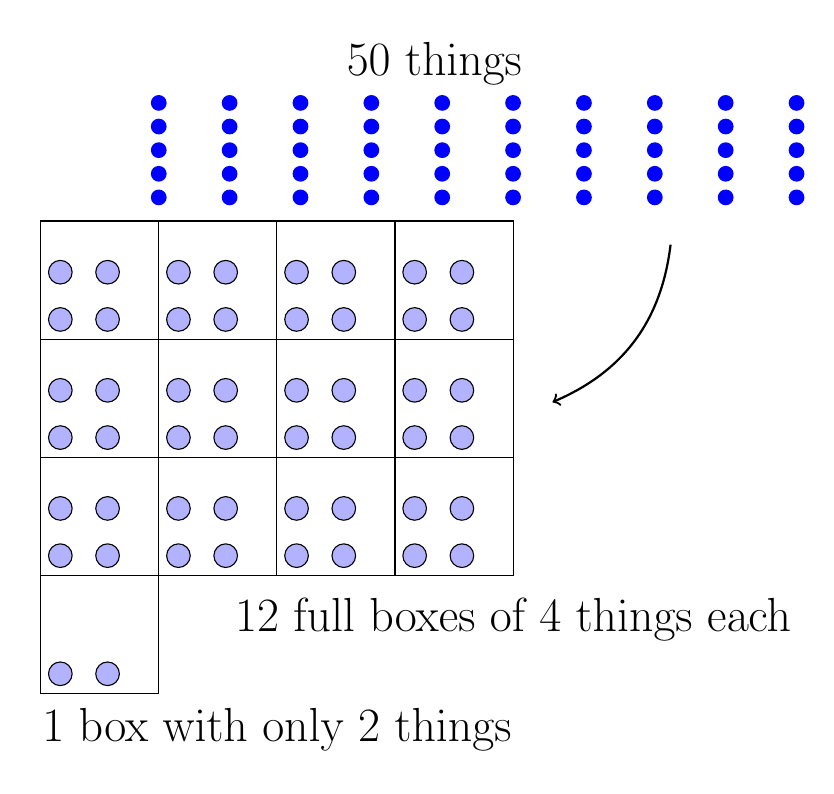
\begin{tikzpicture}
    % Draw 50 small blue circles
    \node at (5, 3.5) {50 things};
    \foreach \i in {0, 1, ..., 9} {
        \foreach \j in {0, 1, 2, 3, 4} {
            \fill[blue] (1.5 + \i*0.9, 3 - \j*0.3) circle (0.1);
        }
    }
    % Draw the curved arrow
    \draw[thick, ->, bend left] (8, 1.2) to (6.5, -.8);
    % Draw the full boxes in a grid of 3 rows and 4 columns
    \foreach \row in {0, 1, 2} {
        \foreach \col in {0, 1, 2, 3} {
            \draw (\col*1.5, -\row*1.5) rectangle +(1.5, 1.5);
            \foreach \j in {0, 1, 2, 3} {
                \pgfmathsetmacro{\xpos}{mod(\j, 2)}
                \pgfmathsetmacro{\ypos}{int(\j / 2)}
                \draw[fill=blue!30] (\col*1.5 + 0.25 + 0.6*\xpos, -\row*1.5 + 0.25 + 0.6*\ypos) circle (0.15);
            }
        }
    }
    % Draw the partially filled box
    \draw (0, -3*1.5) rectangle +(1.5, 1.5);
    \foreach \j in {0, 1} {
        \pgfmathsetmacro{\xpos}{mod(\j, 2)}
        \draw[fill=blue!30] (0.25 + 0.6*\xpos, -3*1.5 + 0.25) circle (0.15);
    }
    % Add labels
    \node[below] at (4*1.5, -3.1) {12 full boxes of 4 things each};
    \node[below] at (3, -4.5) {1 box with only 2 things};
\end{tikzpicture}\\

It is how many times some number "goes into" some other number.\\

How many times does 4 go into 30? 7 times, with 2 left over.\\

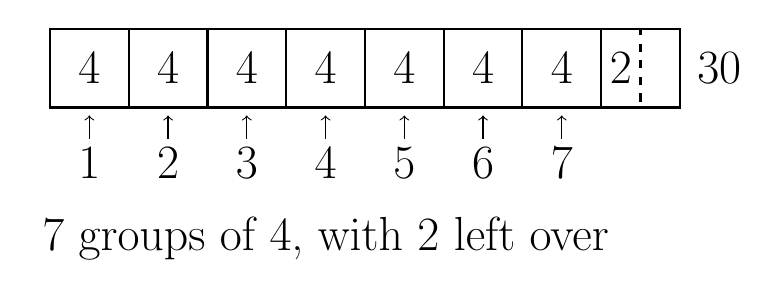
\begin{tikzpicture}
    % Draw the large box representing 30
    \draw[thick] (0,0) rectangle (8, 1);
    \node at (8.5, 0.5) {30};
    % Draw smaller boxes representing groups of 4
    \foreach \i in {0, 1, 2, 3, 4, 5, 6} {
        \draw[thick] (\i*1, 0) rectangle +(1, 1);
        \node at (\i*1 + 0.5, 0.5) {4};
    }
    % Draw the leftover part
    \draw[thick, dashed] (7*1, 0) rectangle +(0.5, 1);
    \node at (7*1 + 0.25, 0.5) {2};
    % Add labels and arrows
    \foreach \i in {1, 2, 3, 4, 5, 6, 7} {
        \draw[<-] (\i*1 - 0.5, -0.1) -- (\i*1 - 0.5, -0.4);
        \node at (\i*1 - 0.5, -0.7) {\i};
    }
    \node[below] at (3.5, -1.2) {7 groups of 4, with 2 left over};
\end{tikzpicture}\\


\item Take a handful of small objects and count them. Now divide them into groups of 4 and count how many groups there are, and how many were left over.

\item Now take those objects and divide them into groups of 3. How many groups are there now? How many are left over?

\item Line your objects up against a ruler and find out how many of them will go into a length of 30 centimetres. What is the length of each object? How many centimetres are left on the ruler that won't fit another object?

\subsubsection*{Dividing into parts of equal sizes}

The other way of dividing is cutting something into equally-sized parts.\\

When division is done this way the size of each part can include a fraction instead of being made up of only whole numbers.\\

Say you had 10 litres of water to share between 4 people. You would pour the water into 4 containers all to the same level, which would be $2\frac{1}{2}$ litres per person.\\

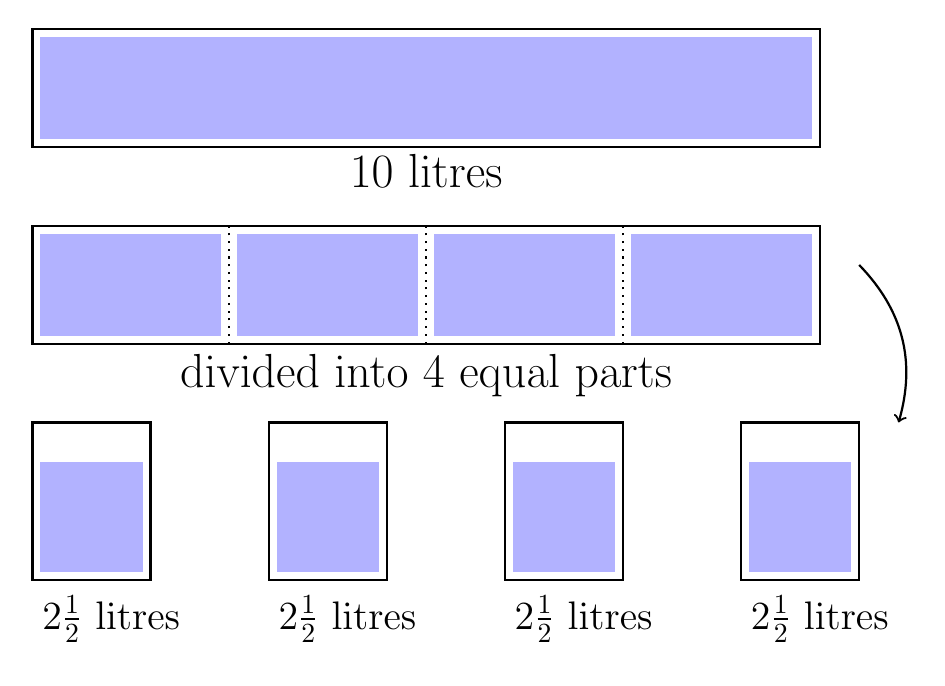
\begin{tikzpicture}
    \draw[thick] (1,1.5) rectangle +(10, 1.5);
    \fill[blue!30] (1.1, 1.6) rectangle +(9.8, 1.3);
    \node at (6, 1.2) {10 litres};

    \draw[thick] (1,-1) rectangle +(10, 1.5);
    \foreach \i in {1, 2, 3} {\draw[dotted, thick] (1 + \i*2.5, -1) -- +(0, 1.5);}
    \foreach \i in {0, 1, 2, 3} {\fill[blue!30] (1.1 + \i*2.5, -0.9) rectangle +(2.3, 1.3);}

    \node at (6, -1.4) {divided into 4 equal parts};
    \draw[thick, ->, bend left] (11.5, 0) to (12, -2);

    \foreach \i in {0, 1, 2, 3} {\draw[thick] (\i*3 + 1, -4) rectangle +(1.5, 2);}
    \foreach \i in {0, 1, 2, 3} {\fill[blue!30] (1.1 + \i*3, -3.9) rectangle +(1.3, 1.4);}
    \node at (2, -4.5) {\small{$2\frac{1}{2}$ litres}};
    \node at (5, -4.5) {\small{$2\frac{1}{2}$ litres}};
    \node at (8, -4.5) {\small{$2\frac{1}{2}$ litres}};
    \node at (11, -4.5) {\small{$2\frac{1}{2}$ litres}};
\end{tikzpicture}\\

\newpage

\item Take some plasticine, roll it into a line, and cut off a piece 10 centimetres long. Now cut it into 4 pieces of the same length. What is the length of each piece?

\item Explain what are the two ways of doing division.
\item Give an example of dividing things in each of the two ways.

\section{Division Symbol}

The symbol for division is "$\div$".\\

Notice that it looks like a fraction but with dots for numbers.\\

Division can also be written with a "/" symbol or it can be written as a fraction. $12 \div 4$ means the same as $12/4$ and it means the same as $\frac{12}{4}$.\\

$$10 \div 4 = 12/4 = \frac{12}{4}$$

\section*{Division Words}

\begin{center}
\textbf{dividend $\div$ divisor = quotient}
\end{center}

\subsection*{Dividend}
The number being divided is called the dividend.\\

\subsection*{Divisor}
The number it is being divided by is called the divisor.\\

\subsection*{Quotient}
The result of division is called the quotient.\\

\item In $6 \div 3 = 2$, which number is the dividend?
\item In $12 \div 4 = 3$, which number is the divisor?
\item In $8 \div 2 = 4$, which number is the quotient?

\newpage

\subsection*{Remainder}
An amount remaining after division is called the remainder.\\

\begin{center}
\small
\textbf{dividend $\div$ divisor = quotient + remainder}\\
$$\textrm{or}$$
\textbf{dividend $\div$ divisor = quotient $\frac{\textbf{remainder}}{\textbf{divisor}}$}\\
\normalsize
\end{center}

The remainder can be written as itself, as in $13 \div 4 = 3$, remainder $1$, or it can be written as a fraction, as in $13 \div 4 = 3 \frac{1}{4}$.\\

To write a remainder as a fraction, write a fraction with the remainder on top and the divisor on the bottom.\\

\item What is $7 \div 8$? Write the answer with a whole number for the remainder and then write the same answer using  a fraction for the remainder.

\newpage

\subsection*{Division and Multiplication}

\subsubsection{Subtraction undoes Addition}
If you add 1 and 5 and then subtract 5 again then you are left with the original 1.

$$1+5=6$$
$$6-5=1$$

\subsubsection{Addition undoes Subtraction}
If you take 5 from 6 and then add it back again then you are left with the original 6.

$$6-5=1$$
$$1+5=6$$

\subsubsection{Multiplication is Repeated Addition}

Multiplication is repeated addition. It is how many times you are adding the same number.

$$4 \times 3 = 12 \textrm{ means } 0\overbrace{+ 4 + 4 + 4}^{\textrm{3\ times}} = 12$$

\subsubsection{Division is Repeated Subtraction}

Division is repeated subtraction. You keep taking an amount away until there's none left.\\

$12 \div 4 = 3$ means $12 \underbrace{- 4 - 4 - 4}_{\textrm{3\ times}} = 0$.\\

\subsubsection{Multiplication undoes Division}

Adding and subtracting are opposites so multiplying and dividing are also opposites.\\

If you divide by a number then multiplying it by that number leaves you with the original number.

$$15 \div 3 = 5$$
$$5 \times 3 = 15$$

\pagebreak

\subsubsection{Division undoes Multiplication}

If you multiply by a number then divide by the same number you are left with the original number.

$$3 \times 2 = 6$$
$$6 \div 2 = 3$$

\item What happens when you subtract the same number that you just added?
\item What happens when you add back the number that you just subtracted?
\item Give an example of how multiplication is repeated addition.
\item Give an example of how division is repeated subtraction.
\item Explain why division and multiplication are opposites.
\item Give an example of multiplication undoing division.
\item Give an example of division undoing multiplication.

\newpage

\section*{Special Rules for Division}
\vspace{16pt}

Any number divided by 1 is unchanged.\\

$$22 \div 1 = 22$$.

Any number divided by itself equals 1.\\

$$22 \div 22 = 1$$.

A number cannot be divided by 0.\\

$$22 \div 0 = \ ???$$

\item What is $65 \div 1$?
\item What is $65 \div 65$?
\item Can $65 \div 0$ be answered?

\pagebreak

\section*{How to Divide}

\subsection*{Using the Multiplication Table}

For smaller numbers it is enough to use the multiplication table to look up the answer for a division.\\

If $7 \times 6 = 42$ then it's easy to look up both $42 \div 6 = 7$ and $42 \div 7 = 6$.\\

\subsubsection{Exercises}

\item On a times table, look up the answer to $49 \div 7$.
\item On a times table, look up the answer to $64 \div 8$.
\item On a times table, look up the answer to $36 \div 4$.

\newpage

\subsection*{Short Division}
Short division is a way of dividing a large number by a single-digit divisor. It is called short division because it is all done on one line.\\

Write the divisor, a right round bracket, and the dividend with a line over it.

\begin{center}
\hspace{3.5em}\textrm{quotient}\\
\mylongdiv{\textrm{divisor}}{\textrm{dividend}}\\
\end{center}

You divide each digit of the dividend, one by one, starting on the left, and writing a digit of the quotient above each digit of the dividend as you go.\\

\newpage

\subsubsection{Procedure}

\begin{itemize}
\item If the divisor is less than or equal to the first digit of the dividend, divide that digit by the divisor and write the quotient above that digit.\\

\item Any remainder is written, small to the left of the next digit of the divisor. It becomes a tens digit to the next digit of the dividend.\\

\item If the divisor is greater than that digit of the dividend then write a 0 above that digit and go to the next digit. Include this next digit of the dividend, do that division, and write the next digit of the quotient above that digit.\\
\end{itemize}

\newpage

\subsubsection{Example}

\begin{center}
\mylongdiv{7}{2,296}\\
\end{center}

In this example, 7 is greater than 2 so include the next digit of the dividend to get 22. $22 \div 7 = 3$ with a remainder of 1. Write the 3 above the 22.
\begin{center}
\hspace{3.5ex}3\\
\mylongdiv{7}{2,296}\\
\end{center}

The remainder is written, small, as a tens digit to the left of the next digit of the dividend.
\begin{center}
\hspace{3ex}3\\
\mylongdiv{7}{2,2{^1}96}\\
\end{center}

Do the same for each digit of the dividend, working from left to right, until the final quotient is reached.\begin{center}
\hspace{5.8ex}3\hspace{0.8ex}2\hspace{0.8ex}8\\
\mylongdiv{7}{2,2{^1}9{^5}6}\\
\end{center}

\newpage

\subsubsection{Exercises}

\item Use short division to solve $147 \div 7$.
\item Use short division to solve $1,652 \div 7$.
\item Use short division to solve $723 \div 3$.
\item Use short division to solve $256 \div 8$.
\item Use short division to solve $40,689 \div 9$.

\newpage

\subsection*{Long Division}
Long division can divide numbers of any length. It is similar to short division where multiples of the divisor are subtracted from parts of the dividend, working from left to right, but the subtractions are written out in full.\\

Write the divisor, a right round bracket, and the dividend with a line over it.\\
 
\begin{center}
\mylongdiv{27}{9,855}\\
\end{center}

27 won't go into 9 but 27 will go 3 times into 98, with a remainder of 17. Write that as a subtraction, with the 3 written above the 98.

\begin{center}
\begin{tabular}{cccccccccc}
 & & & & & &3& & &\\
\cline{4-9}
2&7& &)& &9&8&5&5& \\
 & & & &-&8&1& & & \\\cline{5-7}
 & & & & &1&7& & & 
\end{tabular}
\end{center}

\newpage

Next "bring down" the next digit of the dividend to get a new partial dividend that can now be subtracted from.

\begin{center}
\begin{tabular}{cccccccccc}
 & & & & & &3& & &\\
\cline{4-9}
2&7& &)& &9&8&5&5& \\
 & & & &-&8&1&\downarrow& & \\\cline{5-7}
 & & & & &1&7&5& & 
\end{tabular}
\end{center}

It helps to work out the  multiples of the divisor.\\

\begin{tabular}{c|c|c|c|c|c|c|c|c|c}
 1& 2& 3&  4&  5&  6&  7&  8&  9& 10\\
27&54&81&108&135&162&189&216&243&270
\end{tabular}\\

 Do the subtraction and write the next digit of the quotient above the line.
 
\begin{center}
\begin{tabular}{cccccccccc}
 & & & & & &3&6& & \\
\cline{4-9}
2&7& &)& &9&8&5&5& \\
 & & & &-&8&1& & & \\\cline{5-8}
 & & & & &1&7&5& & \\
 & & & &-&1&6&2& & \\\cline{5-8}
 & & & & & &1&3& & 
\end{tabular}
\end{center}

\newpage

And again, bring down the next digit, subtract the greatest multiple of the divisor that will fit, and write the next digit of the quotient on the line above.

\begin{center}
\begin{tabular}{cccccccccc}
 & & & & & &3&6&5& \\
\cline{4-9}
2&7& &)& &9&8&5&5& \\
 & & & &-&8&1& & & \\\cline{5-8}
 & & & & &1&7&5& & \\
 & & & &-&1&6&2&\downarrow& \\\cline{5-9}
 & & & & & &1&3&5& \\
 & & & & &-&1&3&5& \\\cline{6-9}
  & & & & & & & &0&
\end{tabular}
\end{center}

Now there is no remainder so $9,855 \div 27 = 365$ exactly.

\subsubsection{Exercises}

\item Use long division to solve $252 \div 12$.
\item Use long division to solve $253 \div 23$.
\item Use long division to solve $561 \div 11$.
\item Use long division to solve $2,568 \div 12$.

\pagebreak

\section{Remainders}
Remainders can be expressed just as a remainder, or as a fraction, or as a decimal fraction (a fraction expressed in decimal numbers to the right of the decimal point.)\\

When you reach the last digit of the dividend and there is still a remainder, you get the decimal fraction by adding a decimal point to both the dividend and the quotient, padding the dividend with extra zeroes, and just continuing the procedure.

\begin{center}
\longdivision{675}{12}
\end{center}

The quotient here could be written as 56.25, or as $56 \frac{3}{12}=56 \frac{1}{4}$, or as 56 remainder 3.

\newpage

\subsubsection{Exercises}

\item Use short division to solve $257 \div 4$, expressing the remainder as a decimal fraction.
\item What is that quotient with the remainder expressed as a fraction?
\item Use long division to solve $2,569 \div 16$, expressing the remainder as a decimal fraction.
\item What is that quotient with the remainder expressed as a fraction?

\subsection*{Repeating Decimal Fractions}
The digits of the decimal fraction part of a quotient will either end eventually with no further remainder, or a digit will start to repeat endlessly, or a sequence of digits will start to repeat. That is why it can be better to write a remainder as itself, or as a fraction, rather than as a decimal fraction.\\

When a decimal fraction starts to repeat, that is shown by placing a dot above the repeating digit or by drawing a line above the repeating sequence of digits.\\

You don't keep working out a division past that point.\\

\hspace{12ex} 2 \ 3 . $\dot{8}$\\
\vspace{1pt}
\hspace{10ex} 9\ \overline{ ) \ 2 \ 1 \ ^{3} 5 \ ^8 0 }

\begin{center}
\longdivision{571}{99}
\end{center}\\

\subsubsection{Exercises}

\item Use short division to express $1 \div 3$ as a decimal fraction.
\item Use long division to express $17 \div 11$ as a decimal fraction.

\pagebreak

\section{Checking Division}

To check your answers, rearrange the terms into multiplication instead of division.\\

Say you have worked out that $1,131 \div 87 = 13$. Check your answer by doing $87 \times 13$, which should equal 1,131.\\

If there is a  remainder in your answer, first subtract the remainder from the dividend to make it easily divisible.\\

$12 \div 5 = 2$, with a remainder of 2.\\

$(12 - 2) \times 2 = 10$ means that your answer is correct.\\

\subsubsection{Exercises}

\item Solve $2,736 \div 6$ and then check your answer by multiplication.
\item Solve $2,058 \div 14$ and then check your answer by multiplication.
\item Solve $10,274 \div 4$ and then check your answer by multiplication.

\end{enumerate}

\end{document}
